\chapter{Securitate, testare și validare}

\section{Rolul acestei etape în proiect}

Într-un proiect de tip Favigon, securitatea și validarea nu pot fi tratate ca pași de final adăugați formal. Aplicația gestionează autentificare, sesiuni, proiecte private, upload de fișiere și integrare cu servicii externe costisitoare. În plus, editorul și pipeline-ul AI introduc suficientă complexitate încât o simplă demonstrație vizuală nu este suficientă pentru a susține că produsul este stabil.

Din acest motiv, validarea a fost privită pe trei niveluri:

\begin{itemize}[leftmargin=1.5cm]
  \item \textbf{măsuri preventive în implementare}, care reduc suprafața de risc;
  \item \textbf{testare automată}, concentrată în special pe backend și convertor;
  \item \textbf{validare funcțională}, prin scenarii operaționale și verificări cap-coadă în interfață.
\end{itemize}

\section{Măsuri de securitate implementate}

\subsection{Autentificare și sesiune}

Securitatea începe din zona de autentificare. În Favigon, autentificarea se bazează pe JWT bearer validat în backend, dar transportat către client prin cookie HTTP only. Refresh token-ul este separat și limitat la un path specific. Această alegere reduce expunerea directă a token-urilor în codul client și simplifică rotația lor la refresh \cite{aspnetJwt2025,owaspAuth2026}.

Pentru scenariile de risc mai mare, proiectul include și autentificare în doi pași. Această măsură crește costul unui atac bazat exclusiv pe compromiterea parolei \cite{owaspMfa2026}. Chiar dacă implementarea actuală folosește cod prin email și nu un factor hardware, ea rămâne o îmbunătățire reală față de autentificarea cu un singur factor.

\subsection{Limitarea expunerii API-ului}

O altă măsură importantă este rate limiting-ul configurat diferențiat pe categorii de endpoint-uri. Zona de autentificare are praguri mai stricte, zona AI este limitată pentru a controla costul și abuzul, iar anumite endpoint-uri de utilizatori au propriile reguli. Documentația ASP.NET Core recomandă această abordare pentru protejarea aplicațiilor expuse public \cite{aspnetRateLimiting2025}. În configurația curentă, politicile observabile în \texttt{Program.cs} sunt: \texttt{auth} 10 cereri / minut, \texttt{ai} 10 cereri / minut, \texttt{converter} 30 cereri / minut cu coadă de 2 cereri și \texttt{users} 60 cereri / minut.

În plus, backend-ul impune limite pentru dimensiunea cererilor. Cererile JSON globale au limită de 1 MB, iar endpoint-urile pentru upload sau flush folosesc praguri dedicate de 5 MB, 10 MB și 15 MB, în funcție de tipul operației. Este o măsură simplă, dar utilă împotriva folosirii necontrolate a resurselor.

\subsection{Middleware și antete de securitate}

În \texttt{Program.cs}, backend-ul include middleware personalizat pentru tratarea excepțiilor și middleware pentru antete de securitate. În mediul non-development sunt activate HSTS și redirecționarea HTTPS. CORS este configurat explicit pe baza unei liste de origini permise. Aceste decizii nu fac aplicația invulnerabilă, dar indică o preocupare practică pentru comportamentul în producție \cite{aspnetCors2024,aspnetErrorHandling2025}.

\subsection{Upload-uri și asset-uri}

Proiectul permite încărcarea de imagini pentru profil și pentru proiecte. Din acest motiv, fișierele primite nu sunt tratate ca date neutre. Backend-ul validează tipul, dimensiunea și contextul în care upload-ul este permis. În plus, la actualizarea designului sunt identificate și șterse asset-urile orfane, tocmai pentru a evita acumularea de fișiere inutile.

\begin{table}[H]
  \centering
  \caption{Măsuri de securitate implementate în Favigon}
  \label{tab:masuri-securitate}
  \renewcommand{\arraystretch}{1.2}
  \begin{tabularx}{\textwidth}{>{\RaggedRight\arraybackslash}p{4cm}YY}
    \toprule
    \textbf{Zonă} & \textbf{Măsură implementată} & \textbf{Rol practic} \\
    \midrule
    Autentificare & JWT în cookie HTTP only + refresh token separat & reduce expunerea token-urilor și permite reînnoirea sesiunii \\
    2FA & cod temporar prin email & ridică nivelul de protecție la login și operații sensibile \\
    API public & rate limiting pe politici distincte & reduce abuzul și protejează resursele costisitoare \\
    Transport & HSTS și HTTPS în producție & reduce riscul de trafic neprotejat \\
    Browser/API & CORS configurat explicit & limitează originile care pot face cereri autentificate \\
    Upload-uri & validare de dimensiune și tip & reduce riscul de folosire abuzivă a endpoint-urilor de fișiere \\
    Tratarea erorilor & middleware dedicat pentru excepții & uniformizează răspunsurile și evită scurgeri inutile de detalii \\
    \bottomrule
  \end{tabularx}
\end{table}

\section{Strategia de testare}

Strategia de testare urmărită în proiect a avut două obiective. Primul a fost acoperirea automată a zonelor backend cu risc tehnic mare: autentificare, proiecte, middleware și convertor. Al doilea a fost verificarea cap-coadă a fluxurilor majore, mai ales acolo unde automatizarea completă nu exista încă pe frontend.

La data de 1 iunie 2026, situația observabilă în repository este sintetizată în Tabelul~\ref{tab:indicatori-validare-sinteza}. El arată că validarea actuală este puternic orientată spre backend și spre convertor, în timp ce frontend-ul rămâne relativ slab acoperit automat.

\begin{table}[H]
  \centering
  \caption{Indicatori sintetici ai validării curente}
  \label{tab:indicatori-validare-sinteza}
  \renewcommand{\arraystretch}{1.15}
  \begin{tabularx}{\textwidth}{>{\RaggedRight\arraybackslash}p{6.2cm}Y}
    \toprule
    \textbf{Indicator} & \textbf{Valoare observată} \\
    \midrule
    Teste backend automate trecute & 109 / 109 \\
    Endpoint-uri HTTP expuse de API & 62 \\
    Teste frontend existente în repository & 2 \\
    Coverage backend total (\textit{line coverage}) & 18.33\% \\
    Coverage backend total (\textit{branch coverage}) & 27.79\% \\
    Politici de rate limiting configurate & 4 (auth, ai, converter, users) \\
    Benchmark AI cu prompturi fixe & 5 prompturi, rată de succes 100\%, timp mediu 106.83 s \\
    \bottomrule
  \end{tabularx}
\end{table}

\section{Testare automată backend}

\subsection{Distribuția pe suite}

Rularea locală a comenzii \texttt{dotnet test} pentru proiectul \texttt{Backend/Favigon.Tests} a raportat 109 teste trecute, 0 eșuate și o durată totală de aproximativ 5--6 s. Numărul brut este util, dar mai importantă este distribuția lui pe zone de responsabilitate. În forma actuală, backend-ul nu are o singură suită compactă, ci mai multe suite specializate pe servicii, controllere, middleware și convertor.

\begin{table}[H]
  \centering
  \caption{Distribuția testelor automate backend pe suite}
  \label{tab:distributie-teste-suite}
  \renewcommand{\arraystretch}{1.15}
  \begin{tabularx}{\textwidth}{>{\RaggedRight\arraybackslash}p{4.2cm}Y>{\RaggedLeft\arraybackslash}p{2cm}}
    \toprule
    \textbf{Suită} & \textbf{Zonă verificată în principal} & \textbf{Nr. teste} \\
    \midrule
    Project service & logică de proiecte, fork, like, bookmark, asset-uri & 20 \\
    Converter engine & reguli de export, responsive și multi-page & 11 \\
    Exception handler middleware & tratarea erorilor și maparea excepțiilor & 10 \\
    Projects controller & contractul HTTP pentru proiecte & 11 \\
    Users controller & contractul HTTP pentru utilizatori și profil & 9 \\
    Converter controller & validare și generare prin API-ul convertorului & 9 \\
    User service & operații de profil, follow, search și stări auxiliare & 8 \\
    Auth login & login și stări de acces inițiale & 7 \\
    Security headers middleware & antete de securitate HTTP & 6 \\
    Auth refresh & rotație și validare refresh token & 5 \\
    Auth register & înregistrare și reguli asociate & 5 \\
    Auth password management & parole, resetare și schimbare credențiale & 4 \\
    Auth two-factor & login și operații de administrare 2FA & 4 \\
    \midrule
    \textbf{Total} & \textbf{suită backend automată} & \textbf{109} \\
    \bottomrule
  \end{tabularx}
\end{table}

Privită agregat, distribuția aceasta înseamnă 53 teste de servicii, 29 teste de controllere, 16 teste de middleware și 11 teste pentru motorul de conversie. Pentru proiectul de față, concentrarea este logică: cele mai multe reguli de business și cele mai sensibile transformări se află tocmai în aceste zone.

\subsection{Scenarii reprezentative acoperite automat}

Dincolo de numărul total, este mai util să se observe și ce comportamente sensibile sunt verificate efectiv. Tabelul~\ref{tab:scenarii-teste-reprezentative} rezumă câteva scenarii reprezentative deja ancorate în suitele automate.

\begin{table}[H]
  \centering
  \caption{Scenarii reprezentative verificate prin teste automate}
  \label{tab:scenarii-teste-reprezentative}
  \renewcommand{\arraystretch}{1.15}
  \begin{tabularx}{\textwidth}{>{\RaggedRight\arraybackslash}p{3.4cm}YY}
    \toprule
    \textbf{Zonă} & \textbf{Scenariu testat} & \textbf{Comportament verificat} \\
    \midrule
    Autentificare 2FA & login cu 2FA activ & este emis un token intermediar, se trimite codul și sesiunea finală nu este acordată înainte de verificare \\
    Refresh token & cerere de refresh validă sau invalidă & token-urile sunt reemise corect sau refuzate controlat \\
    Persistență proiect & înlocuirea unui asset imagine & asset-ul vechi nefolosit este eliminat, evitând acumularea de fișiere orfane \\
    Interacțiuni sociale & fork, like și bookmark pe proiecte & relațiile sunt create corect și duplicatele sunt evitate \\
    Export multi-page & normalizarea rădăcinii provenite din canvas & coordonatele specifice editorului nu sunt propagate incorect în CSS-ul exportat \\
    Export responsive & reordonarea copiilor flex pe breakpoint & diferențele de ordine sunt emise în media queries, fără duplicarea inutilă a structurii \\
    Middleware HTTP & excepții și antete de securitate & răspunsurile sunt mapate predictibil și includ antetele așteptate \\
    \bottomrule
  \end{tabularx}
\end{table}

Aceste exemple arată că testarea nu se oprește la cazuri triviale de tip ``200 OK'', ci verifică și comportamente cu miză practică: validarea sesiunilor, controlul fluxului 2FA, curățarea asset-urilor, exportul responsive și middleware-ul de protecție.

\section{Code coverage backend}

Pentru a completa imaginea dată de numărul de teste, a fost rulat și \texttt{dotnet test --collect:"XPlat Code Coverage"}, ceea ce a generat un raport Cobertura pentru proiectele backend. Rezultatul global observat a fost de 18.33\% \textit{line coverage} și 27.79\% \textit{branch coverage}. Luată izolat, această valoare nu este spectaculoasă și trebuie citită cu precauție.

\begin{table}[H]
  \centering
  \caption{Coverage backend pe straturi observat la 1 iunie 2026}
  \label{tab:coverage-backend}
  \renewcommand{\arraystretch}{1.15}
  \begin{tabularx}{\textwidth}{>{\RaggedRight\arraybackslash}p{3.4cm}>{\RaggedLeft\arraybackslash}p{2.6cm}>{\RaggedLeft\arraybackslash}p{2.9cm}Y}
    \toprule
    \textbf{Pachet} & \textbf{Line coverage} & \textbf{Branch coverage} & \textbf{Observație} \\
    \midrule
    Converter & 47.09\% & 34.77\% & cea mai bună acoperire relevantă pentru logica de export \\
    Application & 39.40\% & 27.27\% & acoperire moderată pe serviciile de aplicație \\
    API & 21.86\% & 20.53\% & controllere și rutare verificate parțial \\
    Domain & 58.62\% & 100.00\% & procent mare pe un strat mic, cu logică limitată \\
    Infrastructure & 0.00\% & 0.00\% & practic netestat automat în forma actuală \\
    \midrule
    \textbf{Total backend} & \textbf{18.33\%} & \textbf{27.79\%} & valoarea globală este trasă în jos de zone neacoperite și de ramuri neexercitate \\
    \bottomrule
  \end{tabularx}
\end{table}

Interpretarea corectă a Tabelului~\ref{tab:coverage-backend} este următoarea. Zonele cele mai bine acoperite sunt straturile Converter și Application, exact acolo unde se află reguli tehnice și de business importante pentru lucrare. În schimb, stratul Infrastructure rămâne practic neacoperit automat, iar acest lucru coboară semnificativ scorul global. În consecință, coverage-ul trebuie citit ca indicator de maturitate incompletă, nu ca dovadă că backend-ul ar fi fost testat uniform.

Cu alte cuvinte, proiectul are o bază de teste utilă și bine orientată, dar nu încă una suficient de largă încât să susțină un scor global mare. Prezentarea sinceră a acestei situații este mai valoroasă decât ascunderea ei.

\section{Testare frontend}

Pe partea de frontend, situația este semnificativ mai modestă. În repository există doar un fișier de test, \texttt{app.spec.ts}, care conține două verificări simple la nivelul aplicației. Asta înseamnă că editorul canvas, partea de preview și fluxurile sociale nu au încă o suită automată comparabilă cu backend-ul.

Motivul principal este complexitatea mare a editorului și timpul limitat al proiectului. În locul unei suite largi, dar superficiale, efortul a fost direcționat spre stabilizarea logicii și spre validare funcțională directă. Nu este o soluție ideală pe termen lung, dar pentru stadiul actual al produsului este un compromis explicit. Tocmai de aceea această limită trebuie menționată clar, nu ascunsă în formulări generale despre ``testare suficientă''.

\section{Validare funcțională}

În completarea testelor automate, aplicația a fost verificată prin scenarii funcționale care urmăresc fluxurile principale ale produsului. Acestea includ:

\begin{enumerate}[leftmargin=1.5cm]
  \item creare cont, login și logout;
  \item activare 2FA și autentificare cu pas suplimentar;
  \item creare proiect nou și salvare automată;
  \item editare în canvas cu mutare, redimensionare, selecție și text;
  \item generare AI și integrarea rezultatului în editor;
  \item export în HTML, React și Angular;
  \item publicare, vizualizare publică, like, star și fork.
\end{enumerate}

Această validare a fost utilă mai ales fiindcă a legat împreună subsisteme care, individual, puteau părea corecte. De exemplu, un export poate funcționa separat, dar dacă designul salvat nu este mapat corect în IR, fluxul cap-coadă devine fragil. La fel, 2FA poate funcționa la nivel de API, dar dacă interfața nu tratează bine starea intermediară, experiența utilizatorului se degradează rapid.

\begin{table}[H]
  \centering
  \caption{Scenarii critice și nivelul curent de acoperire}
  \label{tab:scenarii-critice-acoperire}
  \renewcommand{\arraystretch}{1.15}
  \begin{tabularx}{\textwidth}{>{\RaggedRight\arraybackslash}p{5.2cm}cccY}
    \toprule
    \textbf{Scenariu critic} & \textbf{Automat} & \textbf{Funcțional} & \textbf{Neacoperit} & \textbf{Observație} \\
    \midrule
    Login și 2FA & Da & Da & Nu & acoperit prin teste de servicii și verificat cap-coadă \\
    Refresh token și logout & Da & Da & Nu & acoperit automat și observat în interfață \\
    Creare și actualizare proiect & Da & Da & Nu & controller și service acoperite, plus utilizare directă \\
    Upload asset și curățare asset orfan & Da & Da & Nu & verificat atât logic, cât și funcțional \\
    Export HTML / React / Angular & Da & Da & Nu & exportul este testat și folosit în scenarii reale \\
    Generare AI și integrare în editor & Nu & Da & Nu & evaluat prin benchmark și scenarii practice, nu prin teste automate dedicate \\
    Gesturi complexe în canvas & Nu & Da & Nu & validate manual; lipsesc teste frontend bogate \\
    Colaborare simultană în timp real & Nu & Nu & Da & funcționalitatea nu există încă în produs \\
    Load testing pe endpoint-uri AI și converter & Nu & Nu & Da & nu a fost realizată încă o campanie de sarcină \\
    \bottomrule
  \end{tabularx}
\end{table}

Straturile complementare folosite pentru această verificare sunt reprezentate și în Figura~\ref{fig:straturi-validare}.

\begin{figure}[H]
  \centering
  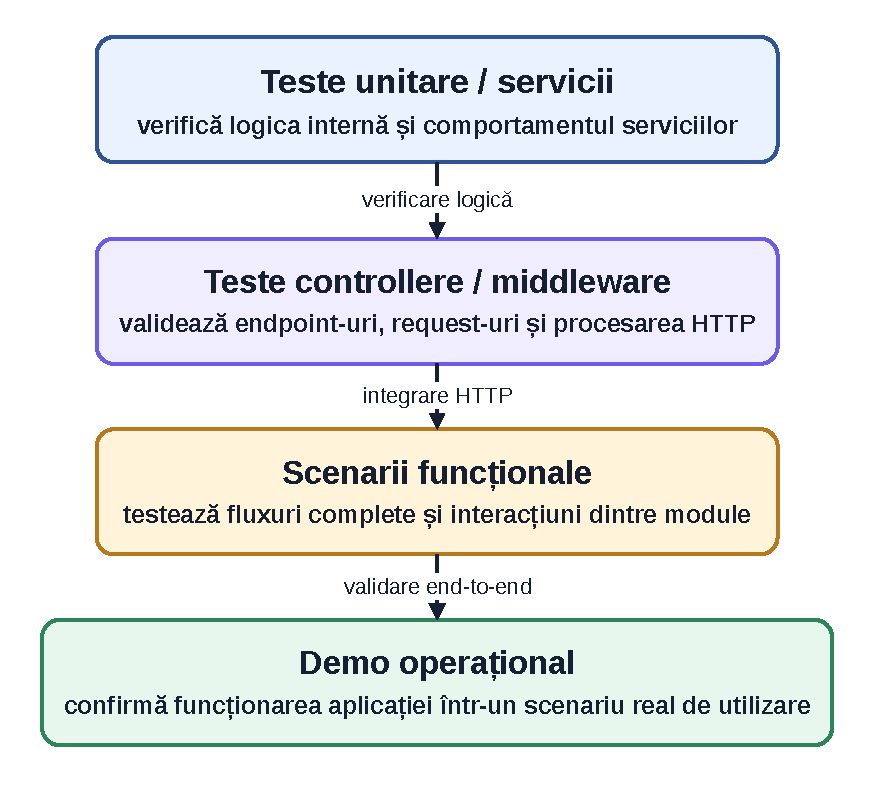
\includegraphics[width=0.78\textwidth]{diagrams/straturi-validare.drawio.pdf}
  \caption{Straturi complementare de validare folosite în proiect}
  \label{fig:straturi-validare}
\end{figure}

\section{Limitări ale testării actuale}

Deși proiectul are o bază bună de verificare, există și limite care trebuie menționate explicit.

Prima limită este testarea frontend-ului. Editorul canvas ar beneficia de teste automate mai bogate, în special pentru interacțiuni complexe, regresii vizuale și scenarii de navigare mai lungi.

A doua limită este partea de AI. Benchmark-ul actual confirmă că pipeline-ul poate produce rezultate valide și exportabile pe un set mic de prompturi, dar nu oferă încă o evaluare largă pe modele multiple, prompturi multiple per categorie sau scenarii de stres.

A treia limită este absența unei campanii complete de load testing. Proiectul are rate limiting și structură tehnică bună, dar nu a fost supus încă unei evaluări cantitative sub sarcină continuă, mai ales pentru endpoint-urile AI și de conversie.

A patra limită este acoperirea redusă a infrastructurii. Chiar dacă \texttt{Infrastructure} este integrată în fluxurile reale de utilizare, ea nu este deocamdată exercitată suficient prin teste automate dedicate.

\section{Concluzii intermediare}

Securitatea și validarea din Favigon nu rezolvă toate problemele posibile, dar oferă o bază credibilă pentru funcționarea produsului. Autentificarea, 2FA, limitarea cererilor, validarea upload-urilor și middleware-ul de protecție reduc riscuri concrete. În paralel, cele 109 teste backend, coverage-ul măsurat explicit și scenariile funcționale arată că proiectul nu este doar conceptual coerent, ci și suficient de bine verificat pentru o lucrare de licență.

În același timp, cifrele arată clar și unde produsul rămâne incomplet: frontend-ul este slab acoperit automat, \texttt{Infrastructure} este practic netestată prin suite dedicate, iar evaluarea AI trebuie extinsă în viitor prin benchmark-uri mai largi și prin măsurători sub sarcină. Tocmai această combinație dintre puncte tari și limite reale pregătește terenul pentru capitolul final.
